This chapter describes all the machines which are going to be used to verify our parameters in detail.
The description of the machines can be found on the HKUST NFF website\footnote{\url{http://www.nff.ust.hk/en/equipment-and-process/equipment-list.html}}, but all the info is being copied over for the benefit of future reproducibility, in case it is decided to by HKUST in the future to take the page down or restrict the access to the information.

\begin{figure}[H]
	\centering
	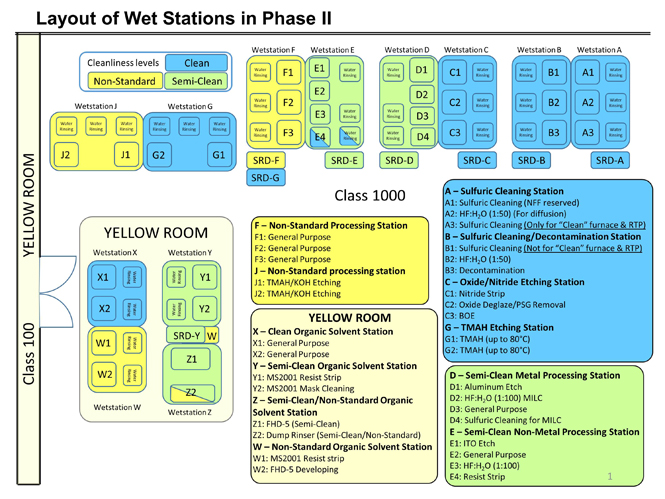
\includegraphics[scale=2]{pictures_machines/wetstations_phase2.png}
	\caption{Wet station map}
	\label{wet_station_map}
\end{figure}

In order to avoid contamination of different cleaniness-class areas (clean, semi-clean, non-standard) we have to track the cleaniness level of the wafer in order to have it move forth and back between the different work station areas.
In \autoref{wet_station_map} we can see the map of the different cleaning stations in order to get our wafer back to clean from non-clean and non-standard so that we can switch forth and back between machines.
